\part{Results}

\begin{frame}
	\partpage
	\centering
\end{frame}

%%%%%%%%%%%%%%%%%%%%%%%%%%%%%%%%%%%%%%%%%%%%%%%%%%%%%%%%%%%%%%%%%%%%%%%%%%%%%%%%%%%%%%%%%%%%%%%%%%%%%%%%%%%%%%%%%%%%%%%%%%%
%%%%%%%%%%%%%%%%%%%%%%%%%%%%%%%%%%%%%%%%%%%%%%%%%%%%%%%%%%%%%%%%%%%%%%%%%%%%%%%%%%%%%%%%%%%%%%%%%%%%%%%%%%%%%%%%%%%%%%%%%%%

\begin{frame}
	\frametitle{Source code \& Dataset}
	\centering
	
	Original source code by medvedev group available on:\\
	
	\medskip
	
	https://github.com/medvedevgroup/TwoPaCo \\
	
	\medskip
	
	$\_\_\_\_\_\_\_\_\_\_\_\_\_\_\_\_\_\_\_\_\_\_\_\_\_\_\_\_\_\_\_\_$ \\
	
	\medskip

	Personal implementation available on:\\
	
	\medskip
	
	https://github.com/GaspareG/TwoPaCo
	
	\medskip
	
	$\_\_\_\_\_\_\_\_\_\_\_\_\_\_\_\_\_\_\_\_\_\_\_\_\_\_\_\_\_\_\_\_$ \\

	\medskip
		
	Dataset for experiments:

	\medskip
	
	5 humans (from human reference genome)\\
  8 primates (from ...)\\
	62 Escherichia coli (from ...)\\
  100 simulated human (from ...)\\
	
	
\end{frame}

%%%%%%%%%%%%%%%%%%%%%%%%%%%%%%%%%%%%%%%%%%%%%%%%%%%%%%%%%%%%%%%%%%%%%%%%%%%%%%%%%%%%%%%%%%%%%%%%%%%%%%%%%%%%%%%%%%%%%%%%%%%
%%%%%%%%%%%%%%%%%%%%%%%%%%%%%%%%%%%%%%%%%%%%%%%%%%%%%%%%%%%%%%%%%%%%%%%%%%%%%%%%%%%%%%%%%%%%%%%%%%%%%%%%%%%%%%%%%%%%%%%%%%%

\begin{frame}
  
	\frametitle{Memory complexity}

  \centering
	
	The memory complexity is the maximum \\ among the first and the second pass of TwoPaCo \\
	
	\medskip
	
	\begin{itemize}
	  \item First pass: insert all $k$-mers in a bloom filter of size $b$
	  \item Second pass: store all \textbf{junction candidates} in a hash table
	\end{itemize}
	
	\medskip
	
	How many junction candidates?
	
	\begin{itemize}
	  \item Real junction, $J$
	  \item False positive induced from the bloom filter, $FP$
	\end{itemize}

	\medskip
	
	Result: $O( \max(b, (J+FP)k) )$
	
	
\end{frame}

%%%%%%%%%%%%%%%%%%%%%%%%%%%%%%%%%%%%%%%%%%%%%%%%%%%%%%%%%%%%%%%%%%%%%%%%%%%%%%%%%%%%%%%%%%%%%%%%%%%%%%%%%%%%%%%%%%%%%%%%%%%
%%%%%%%%%%%%%%%%%%%%%%%%%%%%%%%%%%%%%%%%%%%%%%%%%%%%%%%%%%%%%%%%%%%%%%%%%%%%%%%%%%%%%%%%%%%%%%%%%%%%%%%%%%%%%%%%%%%%%%%%%%%

\begin{frame}
  
	\frametitle{Time complexity}

  \centering
	
	The memory complexity is the sum \\ between the first and the second pass of TwoPaCo \\
	
	\bigskip
	
	\begin{itemize}
	  \item First pass: insert all $k$-mers in a bloom filter of size $b$ using $h$ hash functions
	  \item Second pass: store all \textbf{junction candidates} in a hash table
	\end{itemize}
	
	\bigskip
	
	How many $k$-mers? \\
	
	$O(m)$, where $m = \Sigma_{s \in S}{ |s| }$ is the total input size
	
	\bigskip
	 
	How many junction candidates?
	
	\begin{itemize}
	  \item Real junction, $J$
	  \item False positive induced from the bloom filter, $FP$
	\end{itemize}

	\medskip
	
	Result: $O(mh + (|G_{c}| + FP)k)$
	
	
\end{frame}


%%%%%%%%%%%%%%%%%%%%%%%%%%%%%%%%%%%%%%%%%%%%%%%%%%%%%%%%%%%%%%%%%%%%%%%%%%%%%%%%%%%%%%%%%%%%%%%%%%%%%%%%%%%%%%%%%%%%%%%%%%%
%%%%%%%%%%%%%%%%%%%%%%%%%%%%%%%%%%%%%%%%%%%%%%%%%%%%%%%%%%%%%%%%%%%%%%%%%%%%%%%%%%%%%%%%%%%%%%%%%%%%%%%%%%%%%%%%%%%%%%%%%%%

\begin{frame}
	\frametitle{Performance comparison}
	
	\centering
	
	%\pause
	
	  Previous approach to the problem:
	
	  \begin{itemize}
	    \item Sibelia (St. Petersburg University, RU, 2012)
	    \item SplitMEM (Stony Brook University, USA, 2014)
	    \item bwt-based (Harbin Institute of Technology, CN, 2016)
	    \item TwoPaCo (The Pennsylvania State University, USA, 2016)
	  \end{itemize}

	%\pause	
	
	  \medskip
	  
	  \begin{tabular}{ r | r | r }
    \hline
    Algorithm  &           Time complexity &        Memory complexity   \\ \hline
    Sibelia    & $O(m)$                    & $O(m)$                     \\
    SplitMEM   & $O(m \log{g})$            & $O(m + |G_{c}|)$           \\
    bwt-based  & $O(m)$                    & $O(m)$                     \\
    TwoPaCo    & $O(mh + (|G_{c}| + FP)k)$ & $O( \max(b, (J+FP)k) )$    \\    
    \hline
    \end{tabular}
    
    \medskip

	%\pause
	
    \begin{itemize}
      \item $m = \Sigma_{s \in S}{ |s| }$, total input size
      \item $g = \max_{s \in S}{ |s| }$, size of the biggest genoma
      \item $J$ and $G_{c}$, number of vertex and edge in the de Bruijn Graph
      \item $b$ and $h$, size of the bloom filter table and number of hash functions
      \item $FP$, number of false positives in first pass
    \end{itemize}
    

\end{frame}

%%%%%%%%%%%%%%%%%%%%%%%%%%%%%%%%%%%%%%%%%%%%%%%%%%%%%%%%%%%%%%%%%%%%%%%%%%%%%%%%%%%%%%%%%%%%%%%%%%%%%%%%%%%%%%%%%%%%%%%%%%%
%%%%%%%%%%%%%%%%%%%%%%%%%%%%%%%%%%%%%%%%%%%%%%%%%%%%%%%%%%%%%%%%%%%%%%%%%%%%%%%%%%%%%%%%%%%%%%%%%%%%%%%%%%%%%%%%%%%%%%%%%%%

\begin{frame}
	\frametitle{Fixed memory}
	\centering
	
	How many rounds do we need to compress the graph\\ without exceeding a given memory threshold?
	
	\bigskip
	
	\begin{tabular}{ | r | r | r | r | r | }
  \hline
  Threshold  & Used memory & Bloom filter size & Running time & Rounds \\ \hline
        10GB &      8.62GB &       8.59GB ($2^{33}$) &           4h &      1 \\
         8GB &      6.73GB &       4.29GB ($2^{32}$) &           7h &      3 \\
         6GB &      5.98GB &       4.29GB ($2^{32}$) &           9h &      4 \\
         4GB &      3.51GB &       2.14GB ($2^{31}$) &          11h &      6 \\
  \hline
  \end{tabular}

\end{frame}

%%%%%%%%%%%%%%%%%%%%%%%%%%%%%%%%%%%%%%%%%%%%%%%%%%%%%%%%%%%%%%%%%%%%%%%%%%%%%%%%%%%%%%%%%%%%%%%%%%%%%%%%%%%%%%%%%%%%%%%%%%%
%%%%%%%%%%%%%%%%%%%%%%%%%%%%%%%%%%%%%%%%%%%%%%%%%%%%%%%%%%%%%%%%%%%%%%%%%%%%%%%%%%%%%%%%%%%%%%%%%%%%%%%%%%%%%%%%%%%%%%%%%%%

\begin{frame}
	\frametitle{Parallel scalability}
	\centering
	
	How does the performance of TwoPaCo improve \\to the increasing of working threads?
	 
	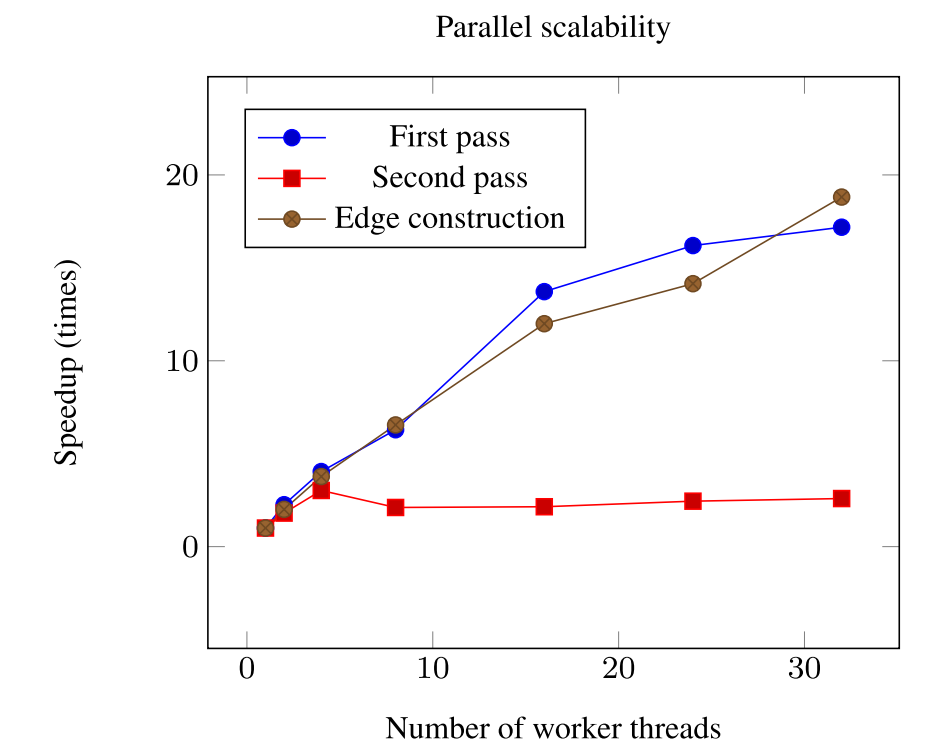
\includegraphics[height=5cm]{images/scalability}
	
	\begin{itemize}
	  \item First pass: great improvement thanks to concurrent bloom filter
	  \item Second pass: slight improvement due to race-conditions on the hash table
	  \item Edge construction: great improvement thanks to $k$-mers independency
	\end{itemize}
\end{frame}

%%%%%%%%%%%%%%%%%%%%%%%%%%%%%%%%%%%%%%%%%%%%%%%%%%%%%%%%%%%%%%%%%%%%%%%%%%%%%%%%%%%%%%%%%%%%%%%%%%%%%%%%%%%%%%%%%%%%%%%%%%%
%%%%%%%%%%%%%%%%%%%%%%%%%%%%%%%%%%%%%%%%%%%%%%%%%%%%%%%%%%%%%%%%%%%%%%%%%%%%%%%%%%%%%%%%%%%%%%%%%%%%%%%%%%%%%%%%%%%%%%%%%%%

\begin{frame}
	\frametitle{Bloom Filter false positive}
	\centering
	
	  Is the Bloom Filter really useful in reducing junction candidates?
	  
    \bigskip
	  
    \begin{tabular}{ r | r | r | r | r | r }
    \hline
    Dataset    &   k &            Initial &       First pass &      Second pass & \%Fp \\ \hline
    62 E.coli  &  25 &  $3.101 * 10^{8\phantom{0}}$  & $2.464 * 10^{7}$ & $2.457 * 10^{7}$ & \phantom{0}0.31\% \\
    62 E.coli  & 100 &  $3.101 * 10^{8\phantom{0}}$  & $2.284 * 10^{7}$ & $9.492 * 10^{6}$ & 58.45\% \\
    7 humans   &  25 &  $2.120 * 10^{10}$ & $3.489 * 10^{9}$ & $2.974 * 10^{9}$ & 14.78\% \\
    7 humans   & 100 &  $2.120 * 10^{10}$ & $1.374 * 10^{9}$ & $1.882 * 10^{8}$ & 86.30\% \\
    8 primates &  25 &  $2.454 * 10^{10}$ & $5.423 * 10^{9}$ & $5.401 * 10^{9}$ & \phantom{0}0.39\% \\
    8 primates & 100 &  $2.454 * 10^{10}$ & $1.174 * 10^{9}$ & $5.024 * 10^{8}$ & 57.20\% \\ \hline
    \end{tabular}
    
    %\caption{Reduction of junction candidates}
    
    \bigskip
    
    \begin{itemize}
      \item Initial: total number of $k$-mers in dataset
      \item First pass: number of junction candidates (using a bloom filter)
      \item Second pass: real number of junction (using an hash table)
      \item False positive: 100*(First pass - Second pass)/(First pass)
    \end{itemize}
    
\end{frame}
